\section{\ourmethod}
\label{sec:proposed_method}
\cref{fig:2_pipeline} illustrates the overall pipeline of \ourmethod.
In the following sections, we first describe the 4D representation of the human and object (\cref{sec:3.1_representation}).
Subsequently, we describe three stages: video decomposition (\cref{sec:3.2_decomposition}), interaction-aware re-rendering (\cref{sec:3.3_generation}), and 4D HOI optimization (\cref{sec:3.4_optimization}).


\subsection{4D representation}
\label{sec:3.1_representation}
Given a monocular video $X$ of $T$ frames, we reconstruct the motion of the human body and the rigid object over the entire sequence.
We represent the human and object as sets of 3D Gaussians~\cite{kerbl3Dgaussians}, denoted by $\{\Phi_{\text{h},t}\}_{t=1}^{T}$ and $\{\Phi_{\text{o},t}\}_{t=1}^{T}$, which can be rendered into 2D space through a differentiable rasterizer~\cite{yu2024mip}.
Each Gaussian is anchored to a surface point of its base mesh, which allows the Gaussians to be converted into meshes~\cite{nam2026tehor}.


\noindent\textbf{Human representation.}
We represent the human with the SMPL-X body model~\cite{pavlakos2019expressive}, parameterized by the human pose $\theta$, translation $\gamma$, and shape $\beta$.
We attach a set of 3D Gaussians $\Phi_{\text{h}}$ to the canonical SMPL-X mesh.
Following ExAvatar~\cite{moon2024expressive}, $\Phi_{\text{h}}$ is deformed by linear blend skinning driven by $\theta$.


\noindent\textbf{Object representation.}
We represent the object in a canonical space, parameterized by rotation $R$, translation $\mathcal{T}$, and scale $s$.
The 3D object Gaussians $\Phi_{\text{o}}$ are transformed by a similarity transformation driven by $R$, $\mathcal{T}$, and $s$.


\noindent\textbf{Temporal parameterization.}
We parameterize the motion of both the human and object as a cubic B-spline~\cite{de1978practical}, a polynomial curve determined by a set of coefficients defined at sparse time intervals.
Unlike independent per-frame pose parameters, the B-spline assigns shared coefficients to neighboring frames, yielding a smooth motion.
Specifically, we define the overall motion sequence as $\Psi=\{\theta_t,\gamma_t,R_t,\mathcal{T}_t\}_{t=1}^{T}$ and formulate it as $\Psi = \mathbf{B}\mathbf{C}$.
$\mathbf{B}\in\mathbb{R}^{T\times N}$ is a B-spline basis matrix, and $\mathbf{C}\in\mathbb{R}^{N\times D}$ is a coefficient matrix, where $N$ is the number of coefficients and $D$ is the dimension of the motion parameters.
All rotations use the continuous 6D rotation representation~\cite{zhou2019continuity}.


\begin{figure*}[t!]
  \centering
  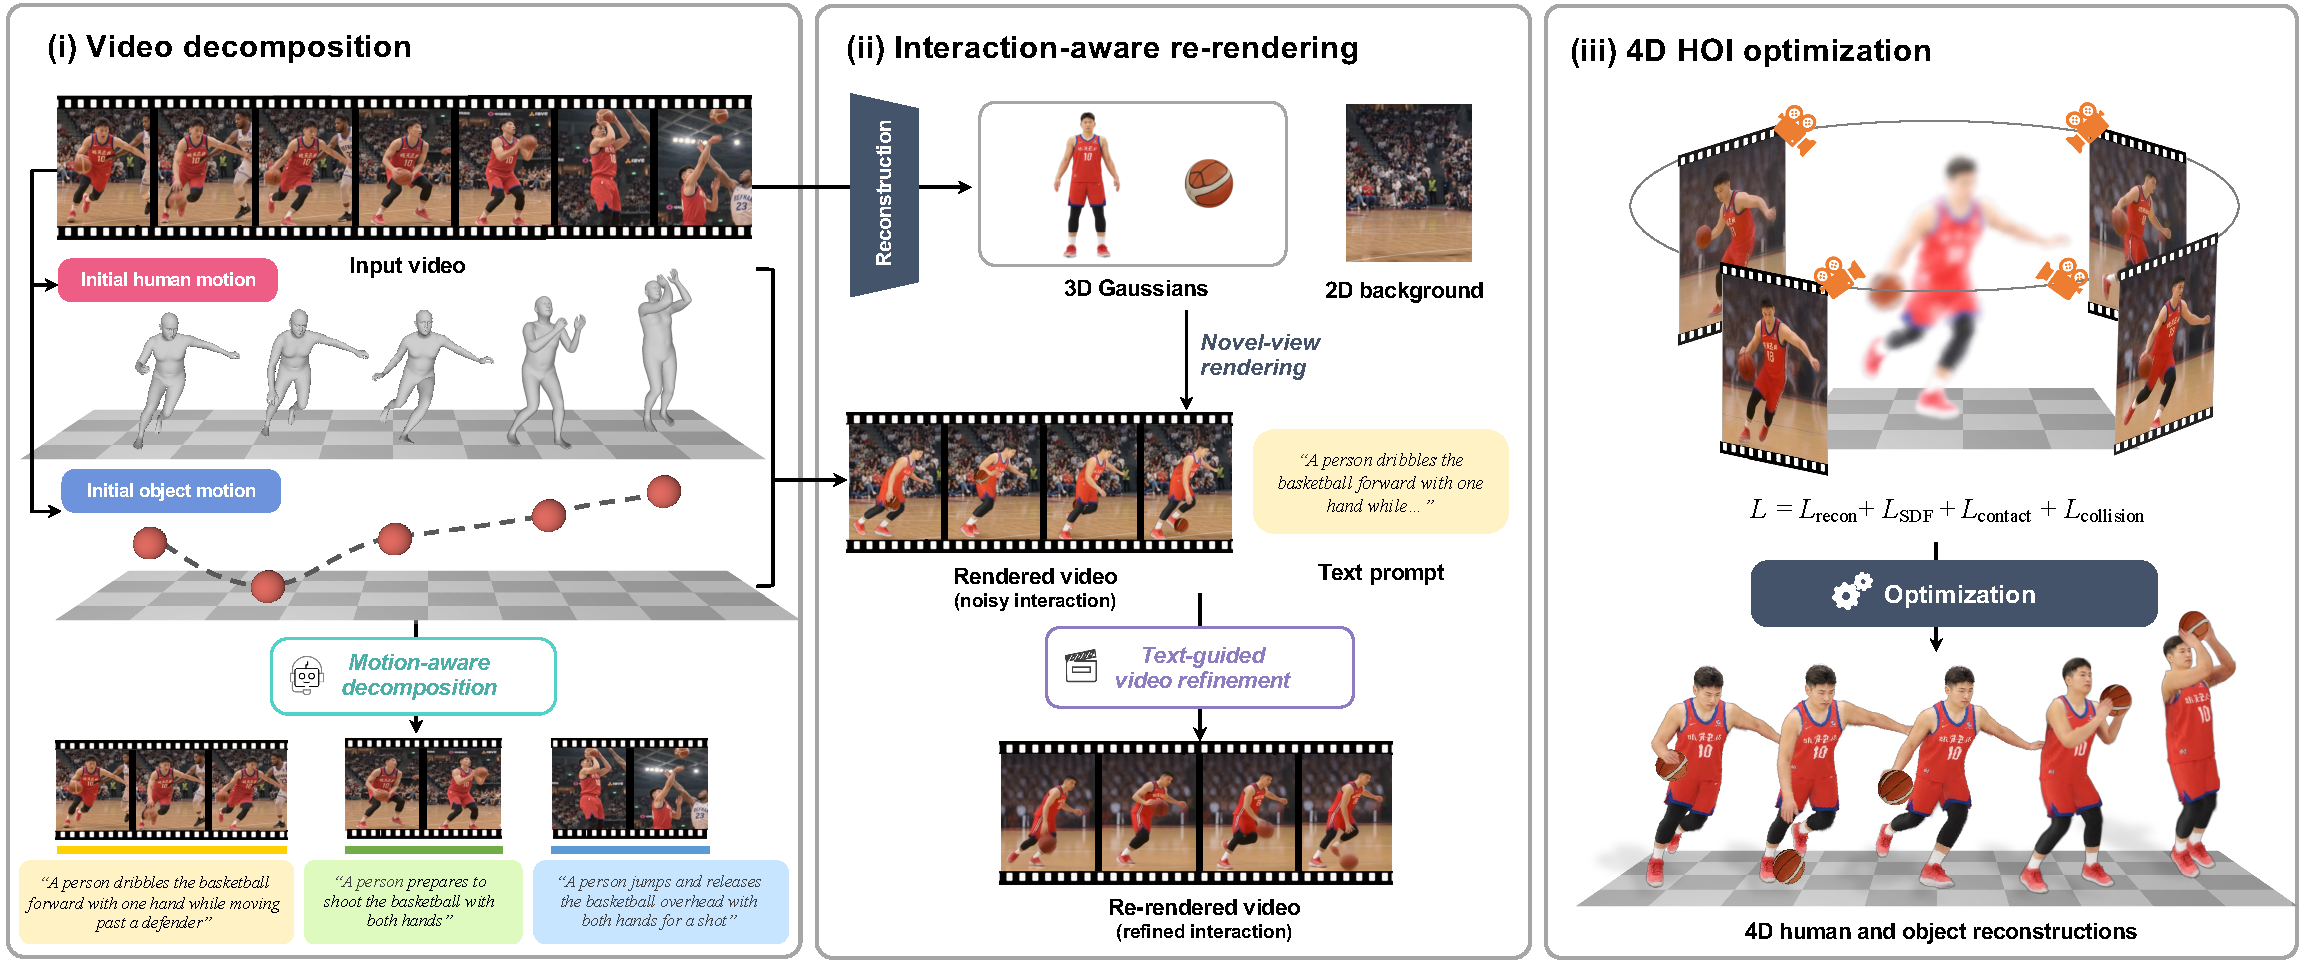
\includegraphics[width=1.0\linewidth]{figures/2_pipeline.pdf}
  \vspace*{-1.65em}
  \caption{\textbf{Overall pipeline of \ourmethod.}
  Given an input video, our framework first decomposes it into temporally grounded sub-actions based on initially estimated human and object motion. 
  Then, the text descriptions of each video segment guide the re-rendering of the human and object under novel viewpoints and provide auxiliary supervision for 4D HOI optimization.
  }
   \vspace*{+0.0em}
  \label{fig:2_pipeline}
\end{figure*}


\subsection{Video decomposition}
\label{sec:3.2_decomposition}
We decompose the input video into sub-action video segments paired with their corresponding text descriptions.
Before the video decomposition, we independently extract the initial motions of the human and object using Multi-HMR~\cite{baradel2024multi} and FoundationPose~\cite{wen2024foundationpose} respectively.
These initial motions serve as physical cues for tracking changes in the relative distance between the human and object over time.
The left panel of \cref{fig:3_pipeline_details} shows the detailed process of decomposing the input video into temporally grounded sub-actions and captioning each of them.


\noindent\textbf{Coarse boundary detection.}
Based on the initial motion estimations, we decompose the input video into sub-actions by identifying boundaries where the interaction state changes.
We first determine coarse temporal boundaries of sub-actions by tracking the object trajectory using the Ramer-Douglas-Peucker (RDP) algorithm~\cite{douglas1973algorithms}.
RDP is a curve simplification method that finds coarse boundaries where the trajectory departs sharply from the overall path.
Such a sharp change in the object trajectory typically coincides with a change in the interaction state, such as the object being picked up, carried, or put down.


\noindent\textbf{Motion-aware captioning.}
From each coarse segment, we extract two text prompts, $P_{\text{semantic}}$ and $P_{\text{contact}}$.
$P_{\text{semantic}}$ captures the global context of the sub-action, providing detailed descriptions of human appearance, object category, and their interaction type.
$P_{\text{contact}}$ specifies the human body parts in physical contact with the object during that interval.
These prompts are acquired using a vision-language model (VLM)~\cite{openai2026gpt5} from five uniformly sampled frames of each coarse segment.
To incorporate 3D human-object distance information in the captioning, we measure the 3D distance between the object and several human parts (\textit{e.g.}, head and hands).
Then, we state whether the object grows \textit{closer}, \textit{farther}, or stays \textit{unchanged} relative to each part from the start to the end of the segment, and provide this information as additional input to the VLM
Detailed descriptions of the motion-aware captioning are provided in supplementary material.


\noindent\textbf{Fine boundary grounding.}
Based on the coarse segments and their text descriptions, we refine the coarse boundaries into precise temporal spans using a temporal grounding model, TimeLens~\cite{zhang2026timelens}.
Specifically, TimeLens queries each caption across the full video timeline to accurately localize the visual extent of each interaction.
If predicted intervals overlap, we merge them into a single continuous segment.
The resulting grounded segments serve as the final sub-action boundaries used for the re-rendering stage (\cref{sec:3.3_generation}).


\subsection{Interaction-aware re-rendering}
\label{sec:3.3_generation}
For each video segment, we generate novel-view interaction videos through re-rendering, which first renders the 3D human and object Gaussians from fixed novel viewpoints and refines the renderings with a text-to-video diffusion network~\cite{wan2025wan}.
To this end, we reconstruct the canonical human Gaussians $\Phi_{\text{h}}$ using LHM~\cite{qiu2025lhm} and the base object Gaussians $\Phi_{\text{o}}$ using SAM 3D~\cite{chen2026sam}, respectively.
We also build a 2D background by removing the human and object from the first frame using SmartEraser~\cite{jiang2025smarteraser}.
The right panel of \cref{fig:3_pipeline_details} illustrates the re-rendering process.


\noindent\textbf{Novel-view rendering and refinement.}
We refine the rendering of the initial human and object reconstructions using a video diffusion prior, providing auxiliary novel-view evidence for the 4D HOI optimization (\cref{sec:3.4_optimization}).
For each novel-view camera $\pi$, sampled at $30^\circ$ azimuth intervals, we render the RGB appearance of the posed human and object Gaussians onto the 2D background to obtain $X_{\pi}$, and project the SMPL-X joints from the same viewpoint to obtain a skeleton video $S_{\pi}$.
We encode $X_{\pi}$ and inject noise to an initial noise level $\tau_0$ to obtain $X_{\tau_0,\pi}$, where the sampling process starts from the rendered appearance.
Conditioned on the sub-action prompt $P_{\text{semantic}}$ and a reference image $X_{\text{ref}}$, which is the first frame of the video segment, we refine $X_{\tau_0,\pi}$ into
\begin{equation}
X^{*}_{\pi} = f_\theta\big(X_{\tau_0,\pi}; P_{\text{semantic}}, S_{\pi}, X_{\text{ref}}\big),
\label{eq:refine}
\end{equation}
where $f_\theta$ denotes a stochastic sampling process~\cite{lipman2023flow} built on a pretrained video diffusion network~\cite{wan2025wan}.
The diffusion network contains rich prior knowledge of realistic human-object interactions, learned from large-scale video data.
Conditioned on the semantic text prompt, the stochastic sampling corrects artifacts associated with implausible human-object interactions, providing reliable novel-view supervision for 4D HOI optimization.


\noindent\textbf{Regional text conditioning.}
To explicitly guide the human and object regions during the refinement, we apply separate text prompts, $P_{\text{human}}$ and $P_{\text{object}}$, to the human mask $M_{\text{human}}$ and object mask $M_{\text{object}}$.
$P_{\text{human}}$ and $P_{\text{object}}$ are extracted from the semantic prompt $P_{\text{semantic}}$.
To capture the contact region, we draw a circular region around the joints of $S_{\pi}$ specified by $P_{\text{contact}}$ and merge it into the object mask $M_{\text{object}}$.
Within every cross-attention layer of the sampling process in \cref{eq:refine}, we blend each region's prompt into the base prompt $P_{\text{semantic}}$ as follows:
\begin{equation}
\text{Attn}^\prime(X_{\tau,\pi}) = \big(1-\beta M_{\text{union}}\big)\,\text{Attn}(X_{\tau,\pi}; P_{\text{semantic}}) + \beta \sum\nolimits_{r} M_r\,\text{Attn}(X_{\tau,\pi}; P_r),
\label{eq:regional_text}
\end{equation}
where $r \in \{\text{human}, \text{object}\}$ indexes the two regions, $M_{\text{union}} = M_{\text{human}} \cup M_{\text{object}}$ is the union of their masks, and $\beta = 0.2$ is a blend weight.
This regional conditioning prevents semantic interference between the human and object while preserving their interaction, providing consistent novel-view supervision for 4D HOI optimization.


\begin{figure*}[t!]
  \centering
  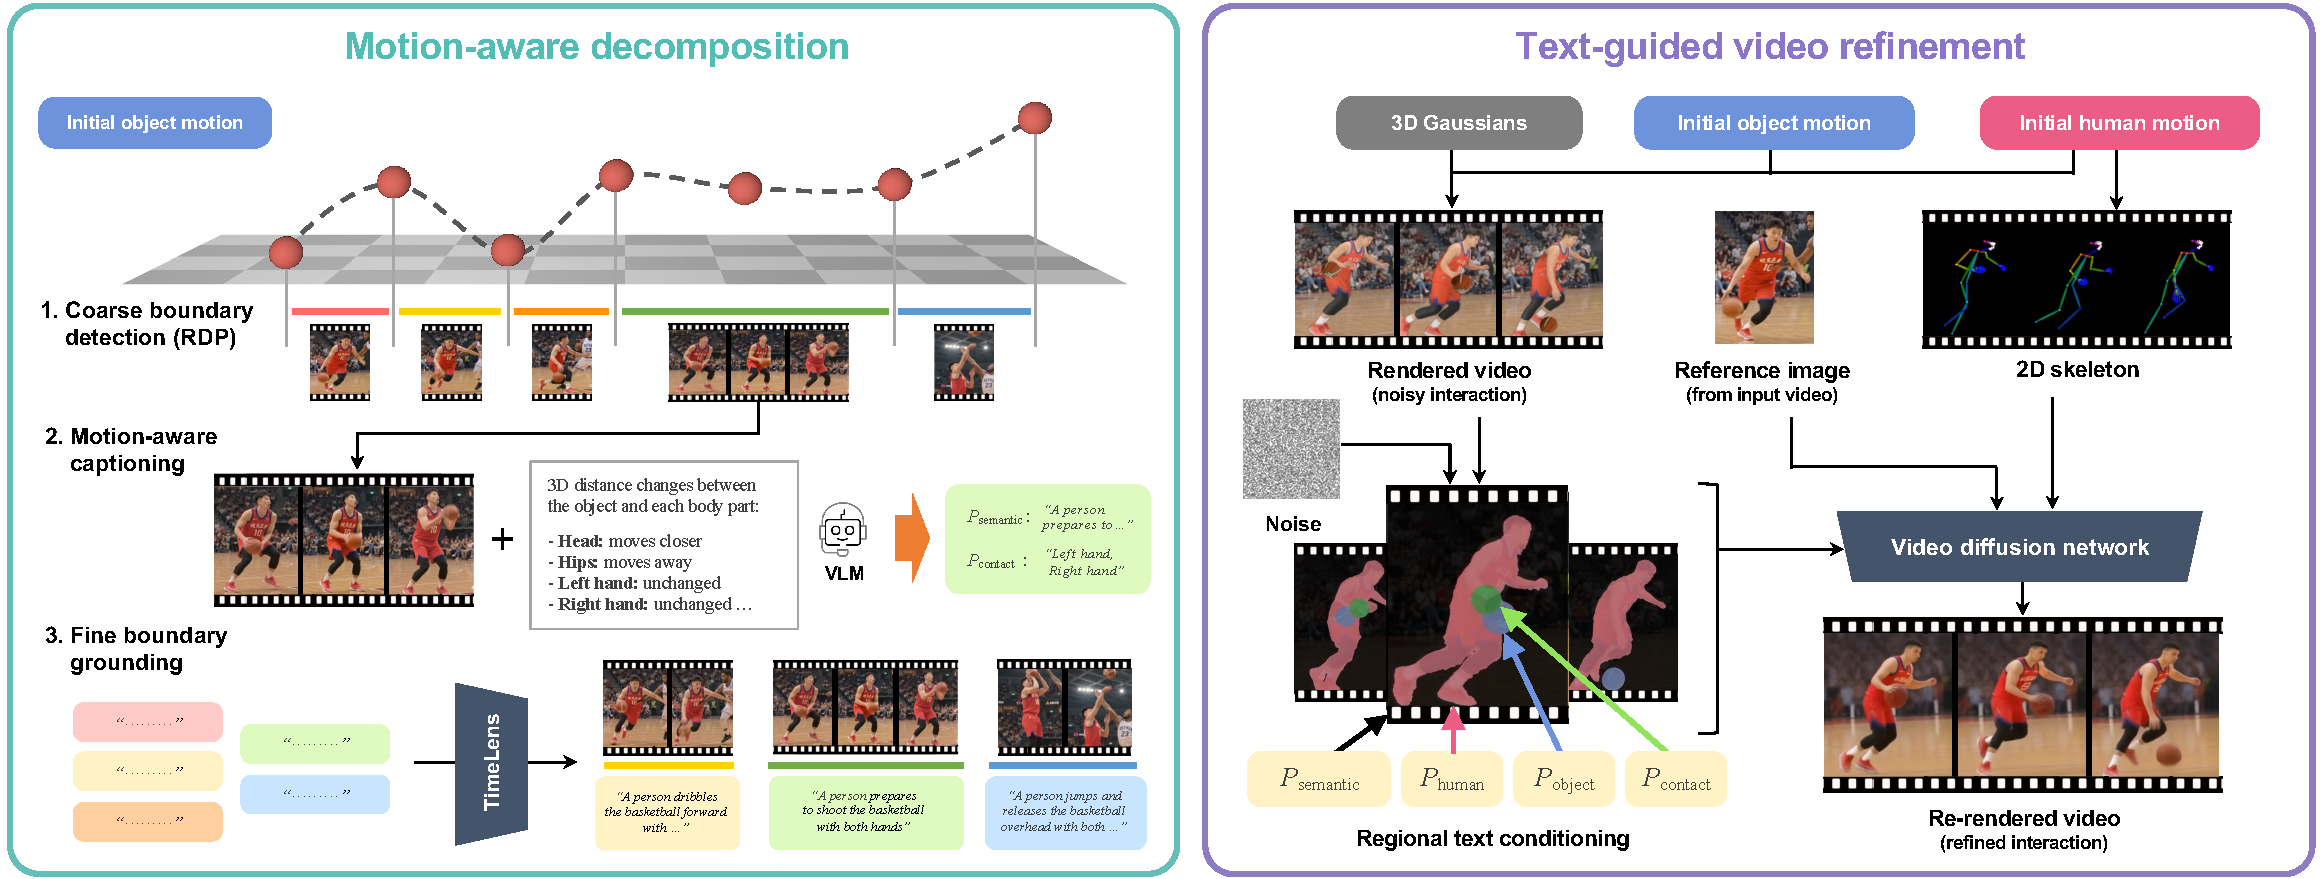
\includegraphics[width=1.0\linewidth]{figures/3_pipeline_detail.pdf}
  \vspace*{-1.6em}
  \caption{\textbf{Detailed process of motion-aware decomposition (left) and text-guided video refinement (right).}
  }
   \vspace*{+0.0em}
  \label{fig:3_pipeline_details}
\end{figure*}


\subsection{4D HOI optimization}
\label{sec:3.4_optimization}
Based on the re-rendered novel-view videos, we jointly optimize the motion sequence $\Psi$ to recover accurate 4D human-object interaction.
The overall loss formulation is
\begin{equation}
\label{eq:overall_loss}
\mathcal{L}=\mathcal{L}_{\text{recon}}+\mathcal{L}_{\text{SDF}}+\mathcal{L}_{\text{contact}}+\mathcal{L}_{\text{collision}},
\end{equation}
where $\mathcal{L}_\text{collision}$ is a penalization term that discourages interpenetration between the human and object Gaussians, following \cite{jiang2020coherent}.
The remaining terms are detailed below.


\noindent\textbf{Reconstruction loss.}
The reconstruction loss $\mathcal{L}_{\text{recon}}$ measures the discrepancy between the rendered human and object sequence and two types of target videos: the input video $X$ and the re-rendered novel-view videos $X^{*}_{\pi}$.
Specifically, it computes the mean squared error (MSE) on both RGB pixel values and foreground silhouette masks across all camera viewpoints.


\noindent\textbf{SDF loss.}
The signed distance function (SDF) loss $\mathcal{L}_{\text{SDF}}$ enforces geometric consistency by aggregating the novel-view evidence into a single 3D point cloud for each frame.
As the novel-view re-rendering (\cref{sec:3.3_generation}) operates on each viewpoint independently, relying solely on $\mathcal{L}_{\text{recon}}$ can result in inconsistent visual cues across views.
To resolve the cross-view inconsistency, we construct a unified 3D geometric consensus across all viewpoints via an SDF.
Specifically, we extract object segmentation masks~\cite{ravi2025sam} and metric depth maps~\cite{piccinelli2024unidepth} from each re-rendered video $X^{*}_{\pi}$ and unproject the masked depth maps into 3D space across all views.
We then aggregate the point clouds and remove outliers via DBSCAN clustering~\cite{ester1996density}, suppressing noisy points inconsistent with the majority of views.
From the point cloud, we build a distance field and align the object Gaussians with the field.
We apply this loss to the object Gaussians only.


\noindent\textbf{Contact loss.}
The contact loss $\mathcal{L}_{\text{contact}}$ encourages geometric proximity between the object surface and the human body parts specified in $P_{\text{contact}}$.
We identify the Gaussian centers on the SMPL-X body model corresponding to these parts and minimize the distance between them and their nearest object points within a predefined threshold.
This loss enforces local physical plausibility across the estimated interaction regions.


\begin{table}[t]
\centering
\footnotesize
\renewcommand{\tabcolsep}{1.0mm}
\def\arraystretch{1.55} % 양쪽 표 모두 동일한 행간 적용

% ==================== Table 1: Decomposition (5행) ====================
\begin{minipage}[t]{0.48\textwidth}
\centering
\caption{
\textbf{Effect of video decomposition.}
}
\label{tab:abl_decomposition}

\vspace{+0.5em}
\scalebox{0.55}{
\begin{tabular}{
>{\centering\arraybackslash}m{2.6cm}
>{\centering\arraybackslash}m{2.1cm}|
>{\centering\arraybackslash}m{0.9cm}
>{\centering\arraybackslash}m{0.9cm}
>{\centering\arraybackslash}m{1.1cm}
>{\centering\arraybackslash}m{1.2cm}
>{\centering\arraybackslash}m{1.1cm}
>{\centering\arraybackslash}m{1.1cm}
}
\specialrule{.1em}{.05em}{0.0em}

Caption
& Decomposition
& CD$_{\text{H}}{\downarrow}$
& CD$_{\text{O}}{\downarrow}$
& Contact${\uparrow}$
& Collision${\downarrow}$ 
& Accel$_{\text{H}}{\downarrow}$
& Accel$_{\text{O}}{\downarrow}$\\
\hline

\xmark      & \xmark    & 5.723 & 54.505 & 0.349 & 0.072 & 0.307 & 3.468 \\
Standard    & \xmark    & 5.500 & 51.155 & 0.391 & 0.059 & 0.291 & 3.129 \\
\textbf{Motion-aware}   & \xmark & 5.511 & 42.102 & 0.408 & 0.060 & 0.294 & 3.210 \\
\textbf{Motion-aware}   & Uniform & 5.404 & 37.121 & 0.469 & \textbf{0.056} & 0.298 & 2.986 \\
\makebox[0pt][c]{\textbf{\;\;\;\;Motion-aware\;\;(Ours)}} & \makebox[0pt][c]{\textbf{Grounded}} & \textbf{5.385} & \textbf{34.894} & \textbf{0.520} & \textbf{0.056} & \textbf{0.273} & \textbf{1.571}\\

\specialrule{.1em}{-0.05em}{-0.05em}
\end{tabular}
}
\end{minipage}
\hspace{0.03\textwidth}%
% ==================== Table 2: Re-rendering (4행) ====================
\begin{minipage}[t]{0.48\textwidth}
\centering
\caption{
\textbf{Effect of re-rendering.}
}
\label{tab:abl_rerendering}

\vspace{+0.5em}
\scalebox{0.55}{
\begin{tabular}{
>{\centering\arraybackslash}m{1.8cm}
>{\centering\arraybackslash}m{2.2cm}|
>{\centering\arraybackslash}m{0.9cm}
>{\centering\arraybackslash}m{0.9cm}
>{\centering\arraybackslash}m{1.1cm}
>{\centering\arraybackslash}m{1.2cm}
>{\centering\arraybackslash}m{1.1cm}
>{\centering\arraybackslash}m{1.1cm}
}
\specialrule{.1em}{.05em}{0.0em}

Re-rendering
& Regional cond.
& CD$_{\text{H}}{\downarrow}$
& CD$_{\text{O}}{\downarrow}$
& Contact${\uparrow}$
& Collision${\downarrow}$ 
& Accel$_{\text{H}}{\downarrow}$
& Accel$_{\text{O}}{\downarrow}$\\
\hline
\xmark   & \xmark       & -- & -- & -- & -- & -- \\
\cmark   & \xmark       & -- & -- & -- & -- & -- \\
\textbf{\cmark\makebox[0pt][l]{\;\;\;\;\;(Ours)}} & \cmark & \textbf{5.385} & \textbf{34.894} & \textbf{0.520} & \textbf{0.056} & \textbf{0.273} & \textbf{1.571}\\
 
\specialrule{.1em}{-0.05em}{-0.05em}
\end{tabular}
}
\end{minipage}

\end{table}

\begin{figure*}[t!]
  \centering
  
\includegraphics[width=1.0\linewidth]{figures/4_optimization_result.pdf}
  \vspace*{-1.5em}
  \caption{\textbf{.}
  }
   \vspace*{+0.0em}
  \label{fig:abl_decomposition}
\end{figure*}
